\documentclass{beamer}

\usepackage[utf8]{inputenc}
\usepackage{tikz}
\usepackage{amssymb}
\usepackage{minted}
\usepackage{natbib}
\usepackage{pdfpages}
\usepackage{listings}
\usepackage{stmaryrd}

\setbeamertemplate{itemize items}[square]

\begin{document}
\title{Rebooting Supercompilation for Haskell}

\author[Ömer\,S.\,Ağacan \& Ryan\,R.\,Newton]
{%
  \texorpdfstring{
    \begin{columns}
      \column{.45\linewidth}
      \centering
      Ömer S. Ağacan\\
      \href{mailto:oagacan@indiana.edu}{oagacan@indiana.edu}
      \column{.45\linewidth}
      \centering
      Ryan R. Newton\\
      \href{mailto:rrnewton@indiana.edu}{rrnewton@indiana.edu}
    \end{columns}
  }
  {Ömer\,S.\,Ağacan \& Ryan\,R.\,Newton}
}

\date{\today}

\frame{\titlepage}

%\frame{\frametitle{Table of contents}\tableofcontents}

\begin{frame}
    \frametitle{Rebooting Supercompilation for Haskell - Talk outline}

    \begin{itemize}[<+->]
        \item
            An overview of supercompilation.
        \item
            What's interesting about it in the context of Haskell? Current
            state-of-the-art.
        \item
            Overview of how it works.
        \item
            "But where's my supercompiler for Haskell?" My preliminary work and
            research goals.
    \end{itemize}
\end{frame}

\begin{frame}[fragile]

    \frametitle{Supercompilation: An overview}

    \begin{itemize}[<+->]
        \item
            Evaluate programs in compile time.
        \item
            Make the most out of known inputs and definitions.
        \item
            Evaluate open terms.
    \end{itemize}

\end{frame}

\begin{frame}
    \frametitle{Supercompilation in the context of Haskell}

    \begin{itemize}
        \item
            Why is it interesting?
        \item
            In a sense, it's the "ultimate" optimization. ("-O99")
        \item
            An evaluator-based supercompiler optimizes in the sense that:

            If we have programs $\mathcal{P}_1$ and $\mathcal{P}_2$, and
            \newline
            $\mathcal{P}_1 \Downarrow v$ in $N$ steps and \newline
            $\mathcal{P}_2 \Downarrow v$ in $M$ steps, \newline
            we consider $\mathcal{P}_2$ optimized if $M \textless N$.
        \item
            An approximation, but works well in practice.
            \newline
            (i.e. if $M \textless N$ then usually $M$ is a faster program)
    \end{itemize}
\end{frame}


\begin{frame}
    \frametitle{Supercompilation in the context of Haskell}

    \begin{itemize}
        \item[]
            It generalizes:
            \begin{itemize}
                \item
                    Deforestation(\citet{deforestation})
                \item
                    Partial evaluation
                \item
                    Call-pattern specialization(\citet{callpatternspec})
                \item
                    Ad-hoc optimizations via rewrite rules, e.g. shortcut fusion
                    (\citet{shortcutdeforestation}) or library-specific rewrite
                    rules
                \item
                    "Optimizing SYB is Easy!"(\citet{optimizingsyb}) and
                    "Optimizing Generics is Easy!"(\citet{optimizinggenerics})
                    style "domain-specific" partial evaluators
                \item
                    Function specialization(\texttt{SPECIALIZE} pragmas)
                \item
                    ... and many more
            \end{itemize}
    \end{itemize}
\end{frame}

\begin{frame}
    \frametitle{Current state-of-the-art for Haskell}

    \begin{itemize}
        \item
            \citet{callbyneed-sc} shows some great potential:
            \begin{itemize}
                \item
                    Up to $20x$ faster runtime.
                \item
                    Up to $100\%$ reduction in allocation.
            \end{itemize}
        \item
            But it also suffers from problems that are inherent to
            supercompilation:
            \begin{itemize}
                \item
                    "We do not attempt to supercompile the full Nofib suite because the
                    other Nofib benchmarks are considerably more complicated and
                    generally suffer from extremely long supercompilation times."
                    \newline
                    (\citet{timeandspace} focuses on compilation performance,
                    and reports \textit{$<$3 seconds} for all the small programs
                    from Nofib)
                \item
                    Up to $132x$ compile time.
                \item
                    Up to $2.8x$ generated code size.
            \end{itemize}
    \end{itemize}
\end{frame}

\begin{frame}
    \frametitle{How it works? An overview}

    \begin{itemize}
        \item[]
            \citet{callbyneed-sc} laid out a great framework for
            supercompiling Haskell:
            \begin{itemize}[<+(1)->]
                \item
                    \textcolor{blue}{Driving:} Take semantics preserving steps.
                    Operational semantics steps, some additional steps like
                    case-of-case
                    transformation(\citet{Jones98atransformation-based}).
                \item
                    \textcolor{blue}{Splitting:} When stuck, keep evaluating
                    sub-expressions. Propagate information. After evaluating
                    sub-expressions combine results.
                \item
                    \textcolor{blue}{Matching:} Evaluating open terms lead to loops.
                    Matcher tries to detect loops, returns information about how
                    to refer to this new loop.
                \item
                    \textcolor{blue}{Termination enforcement:} Because perfect matcher is
                    not possible, and some programs just loop.
            \end{itemize}
    \end{itemize}
\end{frame}

{
    \setbeamercolor{background canvas}{bg=}
    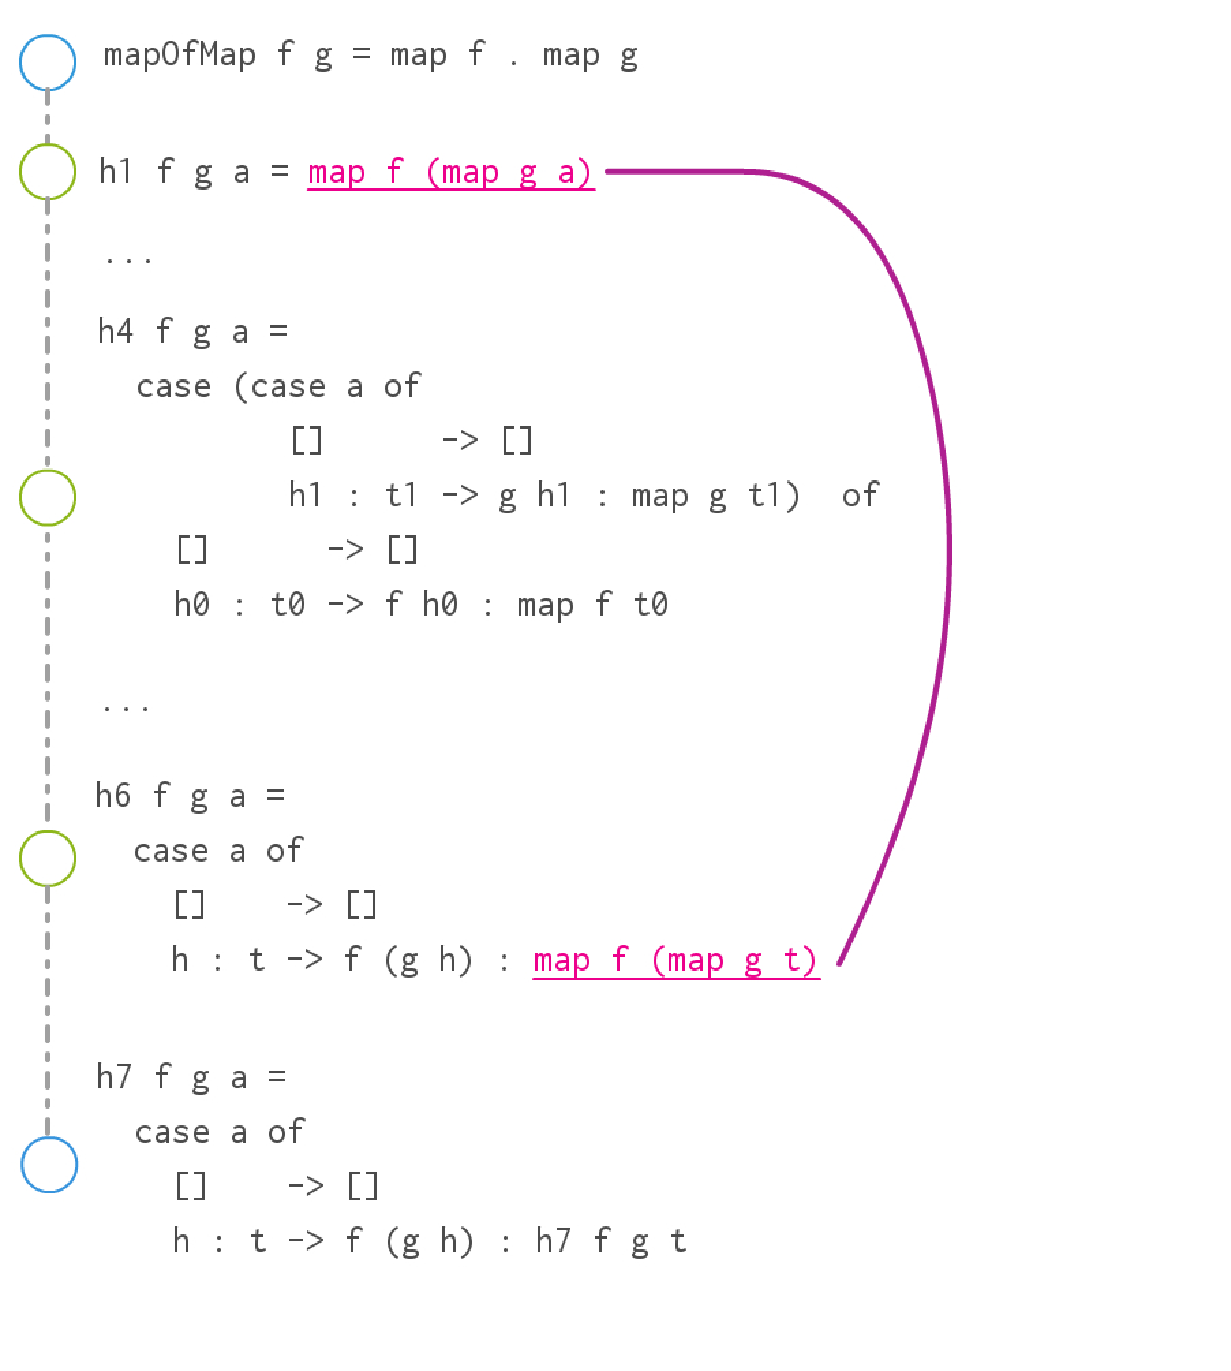
\includepdf[pages={1}]{mapOfMap.pdf}
}

\begin{frame}[fragile]
    \frametitle{Problems with supercompilation operations}

    \begin{itemize}[<+->]
        \item[]
            Each operation has hard problems to solve.

        \item[]
            \textcolor{blue}{Splitter:}
            (from \citet{callbyneed-sc})
            \begin{itemize}
                \item[]
                    Propagating too much information may lead to work
                    duplication.

                    \begin{minted}{haskell}
let n = fib 100
    b = n + 1
    c = n + 2
 in (b, c)
                    \end{minted}
                    \noindent\rule{4cm}{0.4pt}
                    \bigskip
                    \begin{minted}{haskell}
let b =
      let f = <fib, unrolled a few times>
       in f + 1
    c =
      let f = <fib, unrolled a few times>
       in f + 2
 in (b, c)
                    \end{minted}
            \end{itemize}
    \end{itemize}
\end{frame}

\begin{frame}[fragile]
    \frametitle{Problems with supercompilation operations}

    \begin{itemize}
        \item[]
            Each operation has hard problems to solve.

        \item[]
            \textcolor{blue}{Splitter:}
            (from \citet{callbyneed-sc})

            \begin{itemize}
                \item[]
                    Propagating too little information may lead to missing
                    optimization opportunities.
                    \begin{minted}{haskell}
let map = ...
    ys = map f zs
    xs = map g ys
 in Just xs
                    \end{minted}
            \end{itemize}
    \end{itemize}
\end{frame}

\begin{frame}[fragile]
    \frametitle{Problems with supercompilation operations}

    \begin{itemize}
        \item[]
            Each operation has hard problems to solve.

        \item[]
            \textcolor{blue}{Matcher:} Injectivity of substitutions effect
            optimizations.
            \begin{itemize}[<+(1)->]
                \item[]
                    (from \citet{callbyneed-sc})

                    \begin{minted}{haskell}
xor x y = case x of True -> not y; False -> y

goal = (xor a b, xor c c)
                    \end{minted}

                \item[]
                    \centering\noindent\rule{4cm}{0.4pt}
                    \bigskip
                    \begin{minted}{haskell}
xor' x y = case x of True -> not y; False -> y

goal' = (xor' a b, xor' c c)
                    \end{minted}

                \item[]
                    \centering\noindent\rule{4cm}{0.4pt}
                    \bigskip
                    \begin{minted}{haskell}
xor' x y = case x of True -> not y; False -> y

xor'' x = case x of True -> False; False -> False

goal' = (xor' a b, xor'' c)
                    \end{minted}
            \end{itemize}
    \end{itemize}
\end{frame}

\begin{frame}[fragile]
    \frametitle{Problems with supercompilation operations}

    \begin{itemize}

        \item[]
            Each operation has hard problems to solve.

        \item[]
            \textcolor{blue}{Termination enforcement:}

            \begin{itemize}[<+(1)->]

                \item[]
                    Some programs just loop.

                    \begin{minted}{haskell}
loop n = loop (n + 1)
countFrom n = n : countFrom (n + 1)
                    \end{minted}

                \item[]
                    Sometimes detecting loops is not so easy: (growing
                    arguments)

                    \begin{minted}{haskell}
reverse_acc []      acc = acc
reverse_acc (h : t) acc = reverse_acc t (h : acc)
goal lst = reverse_acc (reverse_acc lst []) []
...
h_ lst = ... reverse_acc t1 (h1 : []) ...
...
h_ lst = ... reverse_acc t2 (h2 : h1 : []) ...
...
                    \end{minted}

            \end{itemize}

    \end{itemize}
\end{frame}

\begin{frame}
    \frametitle{"Where's my supercompiler for Haskell?"}

    \begin{itemize}
        \item
            \citet{callbyneed-sc} has some solutions, and it documents and
            implements it nicely.

        \item
            But we still don't have something that we can use \textit{today.}

        \item
            I'm rebooting the supercompiler!

        \item
            The goal here is to distribute it as a package, downloadable from
            Hackage.

        \item
            Then the research will follow.
    \end{itemize}
\end{frame}

\begin{frame}
    \frametitle{Conclusions}

    \begin{itemize}[<+->]
        \item[]
            Have a working implementation of supercompiler described in
            \citet{callbyneed-sc}.
        \item[]
            Collecting benchmark programs - send yours! (with expected
            optimizations)
            \newline
            Create a benchmark suite like Nofib, but for
            supercompilation-specific problems. (pathological cases, programs
            with lots of intermediate data structures)
    \end{itemize}
\end{frame}

\begin{frame}
    Once we have a working implementation:
    \begin{itemize}
        \item
            Focus on specific parts(matcher, splitter etc.). Try other ideas
            from the literature(e.g. homeomorphic embedding for matching)
        \item
            Work on some of the obvious improvements, like parallelizing
            the matcher.
        \item
            More experimental ideas:
            \begin{itemize}
                \item[]
                    Can we formulate it as a search problem and apply ideas from
                    the literature?
                \item[]
                    Is profile-driven decision making possible?
                \item[]
                    Can we make use of existing rewrite rules mechanism?
                \item[]
                    Can we make use of free theorems?
            \end{itemize}
    \end{itemize}
\end{frame}

\begin{frame}
    Once we have a working implementation:
    \begin{itemize}
        \item
            Focus on specific parts(matcher, splitter etc.). Try other ideas
            from the literature(e.g. homeomorphic embedding for matching and
            termination enforcement).
        \item
            Work on some of the obvious improvements, like parallelizing
            the matcher.
        \item
            More experimental ideas:
            \begin{itemize}
                \item[]
                    Can we formulate it as a search problem and apply ideas from
                    the literature?
                \item[]
                    Is profile-driven decision making possible?
                \item[]
                    Can we make use of existing rewrite rules mechanism?
                \item[]
                    Can we make use of free theorems?
            \end{itemize}
    \end{itemize}

    \bigskip
    Thanks!
    \newline
    Github: osa1/sc-plugin \hspace{0.3cm} IRC: osa1 \hspace{0.3cm} Mail:
    oagacan@indiana.edu
\end{frame}

\begin{frame}[allowframebreaks]
    \frametitle{References}

    \bibliographystyle{abbrvnat}
    \bibliography{refs}
\end{frame}

\end{document}
